%============================================================================
% tento soubor pouzijte jako zaklad
% (c) 2008 Michal Bidlo
% E-mail: bidlom AT fit vutbr cz
%============================================================================
% kodovaní: iso-8859-2 (zmena prikazem iconv, recode nebo cstocs)
%----------------------------------------------------------------------------
% zpracování: make, make pdf, make desky, make clean
% připomínky posílejte na e-mail: bidlom AT fit.vutbr.cz
% vim: set syntax=tex encoding=latin2:
%============================================================================
\documentclass[cover]{fitthesis} % odevzdani do wisu - odkazy, na ktere se da klikat
%\documentclass[cover,print]{fitthesis} % pro tisk - na odkazy se neda klikat
%\documentclass[english,print]{fitthesis} % pro tisk - na odkazy se neda klikat
%      \documentclass[english]{fitthesis}
% * Je-li prace psana v anglickem jazyce, je zapotrebi u tridy pouzit 
%   parametr english nasledovne:
%      \documentclass[english]{fitthesis}
% * Neprejete-li si vysazet na prvni strane dokumentu desky, zruste 
%   parametr cover

% zde zvolime kodovani, ve kterem je napsan text prace
% "latin2" pro iso8859-2 nebo "cp1250" pro windows-1250, "utf8" pro "utf-8"
%\usepackage{ucs}
\usepackage[utf8]{inputenc}
\usepackage[T1, IL2]{fontenc}
\usepackage{url}
\usepackage{graphicx}
\usepackage{gensymb}
\DeclareUrlCommand\url{\def\UrlLeft{<}\def\UrlRight{>} \urlstyle{tt}}

%zde muzeme vlozit vlastni balicky


% =======================================================================
% balíček "hyperref" vytváří klikací odkazy v pdf, pokud tedy použijeme pdflatex
% problém je, že balíček hyperref musí být uveden jako poslední, takže nemůže
% být v šabloně
\ifWis
\ifx\pdfoutput\undefined % nejedeme pod pdflatexem
\else
  \usepackage{color}
%  \usepackage[unicode,colorlinks,hyperindex,plainpages=false,pdftex]{hyperref}
  \usepackage[unicode,colorlinks,hyperindex,plainpages=false]{hyperref}
  \definecolor{links}{rgb}{0.4,0.5,0}
  \definecolor{anchors}{rgb}{1,0,0}
  \def\AnchorColor{anchors}
  \def\LinkColor{links}
  \def\pdfBorderAttrs{/Border [0 0 0] }  % bez okrajů kolem odkazů
  \pdfcompresslevel=9
\fi
\fi

%Informace o praci/projektu
%---------------------------------------------------------------------------
\projectinfo{
  %Prace
  project=BP,            %typ prace BP/SP/DP/DR
  year=2012,             %rok
  date=\today,           %datum odevzdani
  %Nazev prace
  title.cs={HAM staniční deník pro Linux},  %nazev prace v cestine
  title.en={HAM logbook for Linux}, %nazev prace v anglictine
  %Autor
  author={Jan Kaluža},   %jmeno prijmeni autora
  %author.title.p=Bc., %titul pred jmenem (nepovinne)
  %author.title.a=PhD, %titul za jmenem (nepovinne)
  %Ustav
  department=UPSY, % doplnte prislusnou zkratku: UPSY/UIFS/UITS/UPGM
  %Skolitel
  supervisor={Václav Šimek}, %jmeno prijmeni skolitele
  supervisor.title.p=Ing.,   %titul pred jmenem (nepovinne)
%   supervisor.title.a={Ph.D.},    %titul za jmenem (nepovinne)
  %Klicova slova, abstrakty, prohlaseni a podekovani je mozne definovat 
  %bud pomoci nasledujicich parametru nebo pomoci vyhrazenych maker (viz dale)
  %===========================================================================
  %Klicova slova
  keywords.cs={HAM, amatérské rádio, deník, klient, server, databáze, C++, Qt, Boost}, %klicova slova v ceskem jazyce
  keywords.en={HAM, logbook, client, server, database, C++, Qt, Boost}, %klicova slova v anglickem jazyce
  %Abstract
  abstract.cs={Cílem této bakalářské práce je navrhout a implementovat staniční deník fungující v systému Linux.
V úvodní části je stručně popsána historie amatérského rádia a objasněny důležité pojmy. Jsou zde taky popsány
aktuálně používané deníky a jejich výhody a nevýhody. Na základě tohoto popisu je proveden návrh aplikace a posléze
také jeho implementace. V závěru je práce zhodnocena a jsou zmíněny možnosti dalšího rozšíření aplikace.
}, % abstrakt v ceskem jazyce
  abstract.en={The goal of this bachelor's thesis is to design and implement an amateur radio logbook for a Linux system.
In the first part there is description of amateur radio history and also a description of important terms used 
between radio amateurs. There are also described currently used applications and their advantages and disadvantages.
Based on this description the logbook application is designed in the second part of this thesis and the concept is
implemented. At the end the application is evaluated and there is a discussion of possibilities for further expansion
of the application.}, % abstrakt v anglickem jazyce
  %Prohlaseni
  declaration={Prohlašuji, že jsem tuto bakalářskou práci vypracoval samostatně pod vedením pana Ing. Václava Šimka.},
  %Podekovani (nepovinne)
%   acknowledgment={Zde je možné uvést poděkování vedoucímu práce a těm, kteří poskytli odbornou pomoc.} % nepovinne
}

%Abstrakt (cesky, anglicky)
%\abstract[cs]{Do tohoto odstavce bude zapsán výtah (abstrakt) práce v českém jazyce.}
%\abstract[en]{Do tohoto odstavce bude zapsán výtah (abstrakt) práce v anglickém jazyce.}

%Klicova slova (cesky, anglicky)
%\keywords[cs]{Sem budou zapsána jednotlivá klíčová slova v českém jazyce, oddělená čárkami.}
%\keywords[en]{Sem budou zapsána jednotlivá klíčová slova v anglickém jazyce, oddělená čárkami.}

%Prohlaseni
%\declaration{Prohlašuji, že jsem tuto bakalářskou práci vypracoval samostatně pod vedením pana X...
%Další informace mi poskytli...
%Uvedl jsem všechny literární prameny a publikace, ze kterých jsem čerpal.}

%Podekovani (nepovinne)
%\acknowledgment{V této sekci je možno uvést poděkování vedoucímu práce a těm, kteří poskytli odbornou pomoc
%(externí zadavatel, konzultant, apod.).}

\begin{document}
  % Vysazeni titulnich stran
  % ----------------------------------------------
  \maketitle
  % Obsah
  % ----------------------------------------------
  \tableofcontents
  
  % Seznam obrazku a tabulek (pokud prace obsahuje velke mnozstvi obrazku, tak se to hodi)
  % \listoffigures
  % \listoftables 

  % Text prace
  % ----------------------------------------------
  \chapter{�vod}

\chapter{Radioamat��i}

\chapter{Rozbor zad�n�}

\chapter{N�vrh aplikace}

C�lem t�to kapitoly pops�n� n�vrhu aplikace a komunika�n�ho protokolu.

Aplikace se skl�d� z modul�rn�ho serveru, klientsk� knihovny a grafick�ho u�ivatelsk�ho rozhran�.
V n�sleduj�c�ch podkapitol�ch jsou jednotliv� ��sti stru�n� pops�ny.

\begin{figure}[h]
\centering
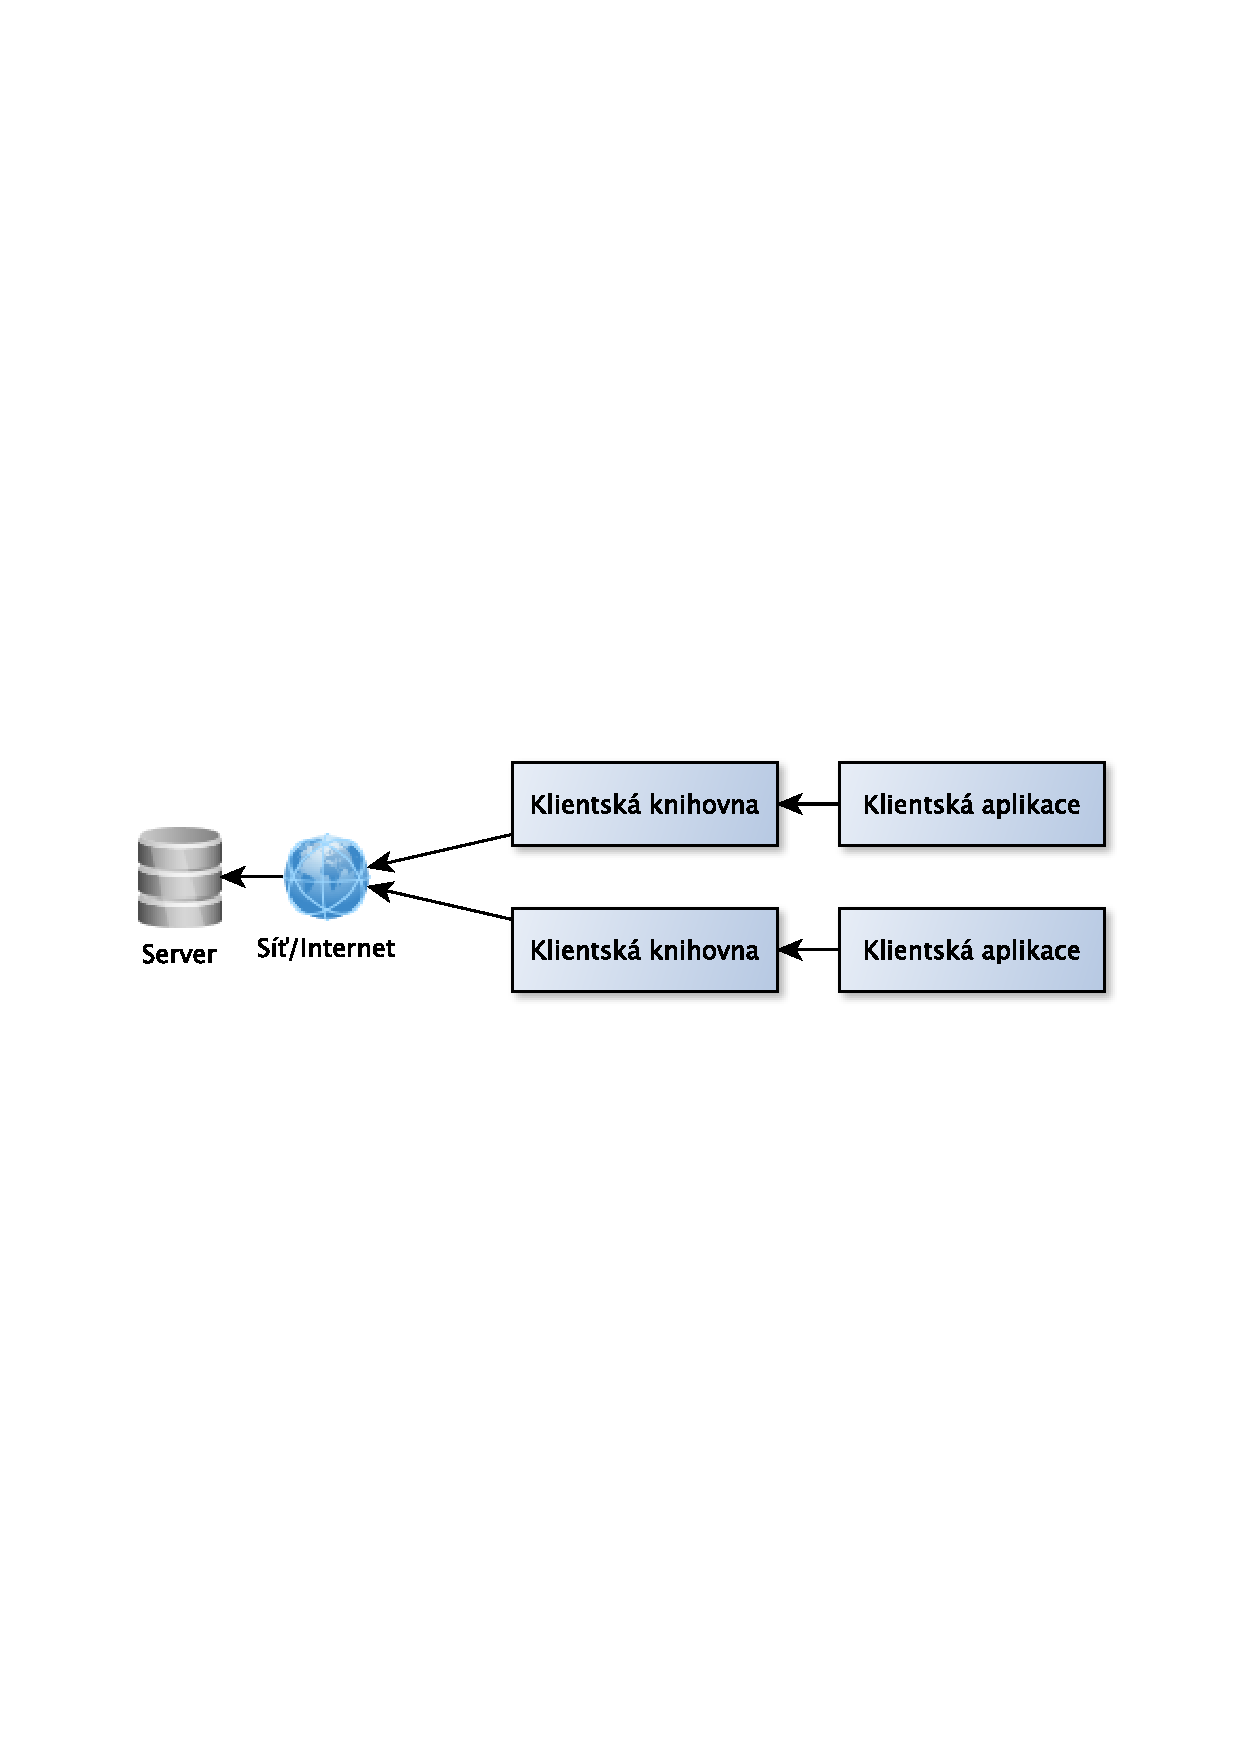
\includegraphics[trim=12cm 12cm 12cm 12cm, scale=0.8]{fig/princip.pdf}
\caption{Z�kladn� �innost programu.}
\label{fig:FigureExample}
\end{figure}

\section{N�vrh komunika�n�ho protokolu}

Byl zvolen protokol inspirovan� protokolem HTTP \cite{http}, p�ev�n� kv�li jeho jednoduchosti a ��elnosti z hlediska modularity.
Jednotliv� moduly serveru maj� sv� vlastn� URI a klientsk� po�adavky jsou pak sm�rov�ny podle URI na konkr�tn� modul,
kter� vygeneruje odpov�� poslanou klientovi.

Protokol je zp�tn� kompatibiln� s protokolem HTTP, ale jsou pou�ity jen n�kter� jeho ��sti.

Data p�en�en� protokolem HTTP jsou ve form�tu CSV \cite{csv}, kde prvn� ��dek reprezentuje hlavi�ku dat.

\subsection{Sch�ma packetu}

Dotaz na modul poskytuj�c� URI "/logbook":
\begin{verbatim}
GET /logbook HTTP/1.1


\end{verbatim}
Odpov�� serveru:
\begin{verbatim}
HTTP/1.1 200 OK
Content-Type: text/hamlog
Content-Length: 74

id;user_id;callsign;date;qth;loc
1;1;TEST;2011;qt;
2;1;LKS;2011;;location
\end{verbatim}

\section{N�vrh serveru}

Server je konzolov� aplikace zpracov�vaj�c� klientsk� po�adavky. Server je schopen obsluhovat v�ce u�ivatel� sou�asn�.
U�ivatel� se k serveru p�ihla�uj� pomoc� jm�na a hesla.
P�ihl�en� je prov�d�no metodou Digest Access Authentication definovanou v RFC 2617. Nov� u�ivatel� se mus� nejprve
registrovat.

N�vrh serveru po��t� s pou�it�m jak�koliv datab�ze pro uchov�n� perzistentn�ch dat. V r�mci t�to bakal��sk� pr�ce jsem se 
rozhodl pou��t datab�zi SQLite3.

Server je modul�rn� a ve�ker� slu�by, kter� u�ivateli poskytuje, jsou sou��st� modul�.

\subsection{Moduly}

Moduly umo��uj� roz�i�ovat dynamicky funk�nost serveru. Ka�d� nov� po�adavek, kter� server od klienta p�ijme je
p�ed�n p��slu�n�mu modulu na z�klad� URI. Modul jej zpracuje a ode�le klientovi zp�t odpov��. Klient si m��e
od serveru vy��dat seznam v�ech modul� pomoc� po�adavku na speci�ln� URI "/modules".

Jednotliv� moduly serveru jsou realizov�ny jako dynamick� knihovny.
P�i spu�t�n� serveru jsou nahr�ny v�echny moduly z adres��e nastaviteln�ho pomoc� konfigura�n�ho souboru.

Ka�d� modul obsahuje n�sleduj�c� informace:

\begin{itemize}
\item URI
\item Typ
\item Popis
\end{itemize}




\section{Klientsk� knihovna}

C�lem klientsk� knihovny je poskytnout grafick�m rozhran�m jednotn� API pro p��stup k serveru
a t�m p�dem zamezit duplikov�n� k�du mezi p��padn�mi grafick�mi rozhran�mi.

Klientsk� knihovna m� minim�ln� z�vislosti a je multiplatformn�.


\section{Klient}

Klient slou�� koncov�mu u�ivateli k p�ipojen� k serveru, prezentaci aktu�ln�ch dat a jejich zm�n�. Pro komunikace
se serverem klient vyu��v� klientskou knihovnu. Pro komunikaci s u�ivatelem pak klient vyu��v� grafick�ho rozhran�.
Po startu klienta je u�ivatel vyzv�n k p�ihl�en� se k serveru. U�ivateli je rovn� nab�dnuta mo�nost registrace
nov�ho ��tu.

Po p�ihl�en� zobraz� klientsk� aplikace ve�ker� z�znamy v den�ku a umo�n� jejich editaci. Klientsk� aplikace tak� zobrazuje
aktu�ln� vys�l�n� z�skan� ze slu�by DXCluster.


\chapter{Implementace}

V t�to kapitole je pops�na implementace serverov� aplikace, klientsk� aplikace a klientsk� knihovny.

\section{Implementace serverov� aplikace}

Server byl implementov�n v jazyce C++ umo��uj�c�m lep�� dekompozici aplikace a pou�it� objektov�ho paradigmatu. Byla rovn�
pou�ita knihovna Boost, kter� poskytuje z�kladn� metody pro asynchronn� s��ovou komunikaci a nab�z� program�torsk� prost�edky
nad r�mec standardn� STL knihovny.

Pro implementaci modulu QRZ bylo pot�eba pou��t knihovnu pro zpracov�n� XML. K tomuto ��elu jsem pou�il knihovnu TinyXML.

\subsubsection{T��da Server}

T��da Server je z�kladn� t��dou serveru. Vytv��� soket, na kter�m server p�ij�m� p�ipojen� z klientsk� knihovny. Jakmile je 
akceptov�no nov� p�ipojen�, je vytvo�ena instance t��dy Session, kter� d�le zpracov�v� v�echny po�adavky klienta.

\subsubsection{T��da Session}

Tato t��da reprezentuje sezen� jednoho u�ivatele. P�i obdr�en� nov�ch dat od klienta jsou tato p�ed�na instanci t��dy
RequestParser, kter� slou�� k jejich rozparsov�n�. Pokud byla obdr�ena kompletn� zpr�va, je p�ed�na instanci t��dy 
ModuleManager metodou handleRequest, kter� pak ��d� jej� dal�� zpracov�n�. V�sledn� odpov�� je pak v t��dou Session posl�na
zp�t klientovi.

\subsubsection{T��da RequestParser}

T��da RequestParser reprezentuje kone�n� automat pro parsov�n� zpr�v podle specifikace komunika�n�ho protokolu.
Metoda parse zpracov�v� p�ijat� data, parsuje je, a v�sledek uchov�v� v instanci t��dy Request. Pokud dojde b�hem parsov�n�
k chyb�, vrac� funkce parse hodnotu false.

\subsection{Implementace datab�zov�ho rozhran�}

N�vrh a implementace serveru umo��uje pou�it� libovoln�ho datab�zov�ho rozhran�. V r�mci bakal��sk� pr�ce je v�ak podpov�na
pouze datab�ze SQLite3. T��da implementuj�c� konkr�tn� datab�zov� rozhran� mus� d�dit t��du StorageBackend a implementovat
jej� �ist� virtu�ln� metody.

\subsubsection{T��da StorageBackend}

T��da StorageBackend je z�kladn� abstraktn� t��dou pro implementaci jak�hokoliv datab�zov�ho rozhran�.
Je typu singleton a jej�m smyslem je poskytnout rozhran� pro z�sk�v�n� dat z datab�zov�ho rozhran� bez znalosti
o jakou datab�zi se jedn�. N�zvy metod a podt��d jsou pojmenov�ny terminologi� zn�mou z SQL datab�z�, ale prakticky
lze pomoc� t��dy StorageBackend implementovat rozhran� pro p��stup k jak�mukoliv typu datab�ze.

T��da StorageBackend Obsahuje z�kladn� podt��dy pro definici dotaz� typu SELECT, INSERT, UPDATE a CREATE zn�m�ch z
jazyka SQL:

\begin{itemize}
\item StorageBackend::Column - Obsahuje ve�ker� informace o sloupci tabulky (jm�no, typ, velikost,
p��znaky pro NOT NULL, UNIQUE a PRIMARY KEY). Slou�� pro definici sloupce p�i vytv��en�
nov� tabulky metodou StorageBackend::createTable().
\item StorageBackend::Select - Zapouzd�uje data pot�ebn� pro proveden� v�b�ru dat z datab�ze. Obsahuje jm�no tabulky,
ze kter� se v�b�r prov�d�, a ukazatel na dvourozm�rn� pole, do kter�ho se ulo�� v�sledky. D�le umo��uje t��da StorageBackend::Select
definovat omezen� v�b�ru (v SQL jazyce kl��ov� slovo WHERE) a umo��uje v�b�r konkr�tn�ch sloupc�, kter� vr�t� ve v�sledku.
Instance t�to t��dy je p�ed�na metod� StorageBackend::select() nebo StorageBackend::remove().
\item StorageBackend::Insert - Obsahuje data pro vlo�en� (v SQL jazyce INSERT) nebo aktualizaci (v SQL jazyce UPDATE)
z�znamu v datab�zi. Obsahuje n�zev tabulky, ve kter� se budou data m�nit, a samotn� data ve form� n�zev sloupce - hodnota.
Umo��uje definovat omezen� (v SQL jazyce WHERE) aplikovan� p�i aktualizaci dat. Instance t�to t�idy je p�ed�na metod�
StorageBackend::insert() nebo StorageBackend::update().
\end{itemize}

V z�vislosti na implementaci metod t��dy StorageBackend je pak vyvol�na konkr�tn� zm�na v datab�zi. T��da StorageBackend
d�le umo��uje z�sk�n� identifika�n�ho ��sla naposledy vlo�en�ho z�znamu metodou lastInsertedID().


\subsubsection{T��da SQLite3Backend}

Tato t��da d�d� t��du StorageBackend a implementuje jej� metody pro pou�it� datab�zov�ho syst�mu SQLite3. V metod�ch
update(), insert(), select(), createTable() a remove() se na z�klad� p�edan�ch dat vygeneruje dotaz v SQL jazyce, spust� se
a je vr�cen v�sledek.

\subsection{Implementace modul�}

Moduly jsou implementov�ny jako dynamick� knihovny. Ka�d� modul mus� d�dit t��du Modul a implementovat jej� �ist� virtu�ln�
(pure virtual) metody. Ve�ker� klientsk� po�adavky jsou pak sm�rov�ny na konkr�tn� modul podle URI instanc� t��dy ModuleManager.

\begin{figure}[h]
\centering
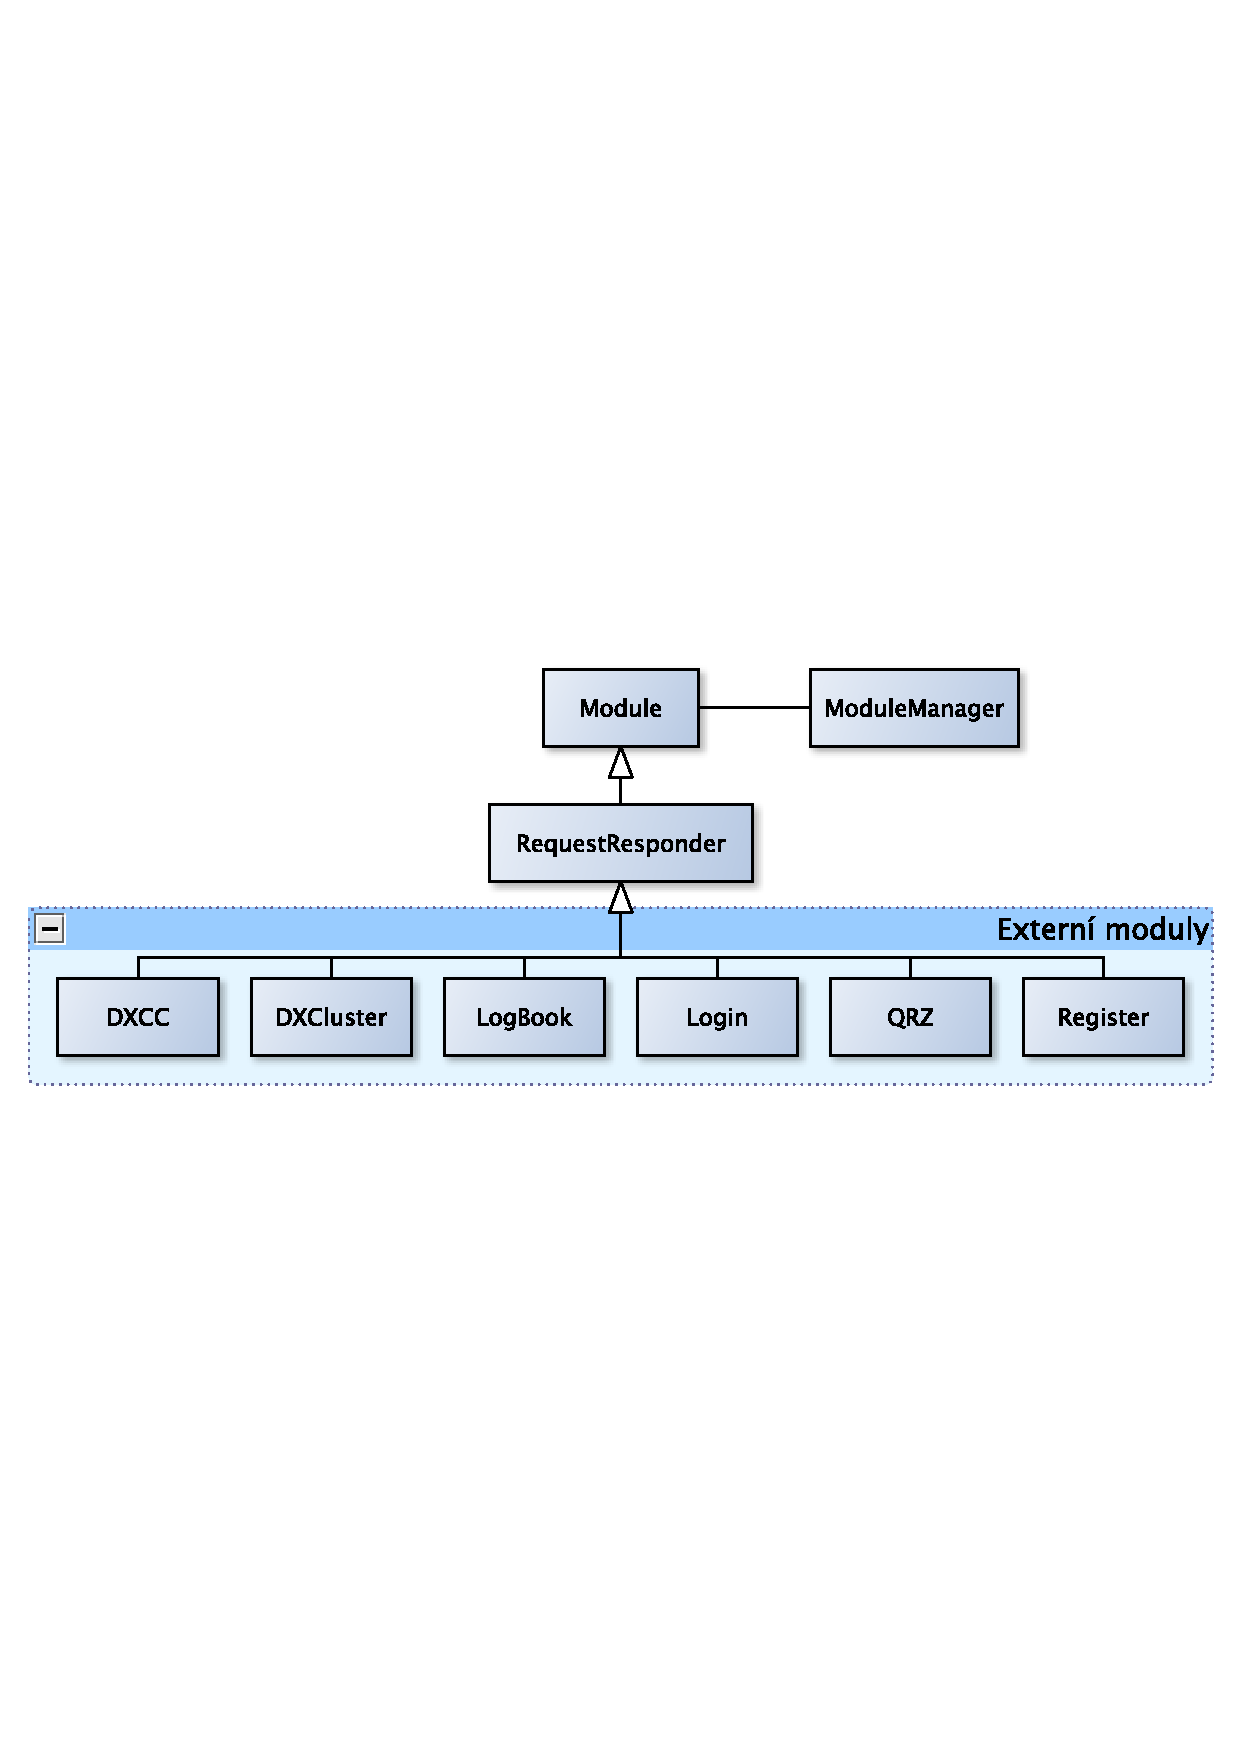
\includegraphics[trim=10cm 10cm 10cm 10cm, scale=0.7]{fig/moduly.pdf}
\caption{Diagram t��d modul�.}
\label{fig:FigureExample}
\end{figure}

\subsubsection{T��da Module}

T��da Module poskytuje z�kladn� t��du, kterou mus� implementovat ka�d� extern� modul. Obsahuje z�kladn� informace o modulu 
(jeho jm�no, typ a popis).

\subsubsection{T��da RequestResponder}

Tato t��da d�d� t��du Module a roz�i�uje ji o data a metody specifick� pro modul odpov�daj�c� na klientsk� po�adavky.
P�i�azuje modulu jeho URI a informaci o tom, jestli mus� b�t u�ivatel pro jeho pou�it� p�ihl�en.
Obsahuje tak� deklaraci metody handleRequest(), kter� je vol�na instanc� t��dy ModuleManager pro ka�d� p��choz� po�adavek
smeruj�c� na modul.

\subsubsection{T��da ModuleManager}

T��da ModuleManager je typu singleton (jedin��ek) a zabezpe�uje ve�kerou pr�ci serveru s extern�mi moduly. Pomoc� 
metody loadModules lze na��st v�echny moduly z adres��e zvolen�ho v konfigura�n�m souboru. Ve�ker� po�adavky od klient�
jsou p�ed�ny instanci t�to t��dy metodou handleRequest, kter� je pak d�le sm�ruje podle URI na konkr�tn� modul. T��da tak�
umo��uje poslat seznam v�ech modul� klientovi.

\subsection{Seznam implementovan�ch modul�}

V t�to podkapitole jsou pops�ny jednotliv� implementovan� moduly.

\subsubsection{Modul Register}

Modul Register (b��c� na URI "/register") slou�� k registraci nov�ch u�ivatel�. P�i sv�m spu�t�n� vytvo�� pomoc�
instance t��dy StorageBackend tabulku "users". V metod� handleRequest pak p�ij�m� p��padn� po�adavky na registraci
u�ivatele a p�id� nov�ho u�ivatele do datab�ze. Pokud je ji� u�ivatel zaregistrov�n, vrac� klientovi chybov� k�d.

\subsubsection{Modul Login}

Modul Login b�� na URI "/login". Jeho c�lem je umo�nit u�ivatel�m p�ihl�en� k syst�mu. V metod� handleRequest je
implementov�n princip p�ihl�en� WWW-Authenticate.

\subsubsection{Modul LogBook}

Tento modul je z�kladem cel�ho projektu, proto�e umo��uje u�ivateli ukl�dat nov� logy na server. P�i sv�m na�ten�
vytvo�� tabulku "logbook". V metod� handleRequest na z�klad� URI prov�d� n�sleduj�c� akce:

\begin{itemize}
\item URI "/logbook" - Jako odpov�d na dotaz po�le cel� logbook v CSV form�tu.
\item URI "/logbook/add" - P�id� do tabulky "logbook" nov� z�znam podle CSV dat p�ijat�ch v dotazu.
\item URI "/logbook/remove" - Odstran� z tabulky "logbook" z�znam definovan� pomoc� ID p�ijat�ho v dotazu.
\item URI "/logbook/call" - Jako odpov�� na dotaz po�le pouze z�znamy s CALL definovanou v CSV datech v dotazu.
\end{itemize}

\subsubsection{Modul DXCC}

Modul DXCC (b�� na URI "/dxcc") umo��uje z�skat z volac� zna�ky bli��� informace o jej� lokaci. Data o jednotliv�ch prefixech
jsou po startu modulu na�tena z souboru "cty.csv" v CSV form�tu. V metod� handleRequest modul z�sk� z po�adavku prefix volac�
zna�ky, vyhled� jej v datech na�ten�ch p�i startu a jako odpov�� ode�le informace o lokaci zna�ky. Pokud prefix nen� nalezen,
vrac� se chybov� k�d.

\subsubsection{Modul DXCluster}

Modul DXCluster (b��c� na URI "/dxcluster") slou�� k p�ipojen� k DXClusteru dxspots.com. P�i prvn�m po�adavku od klienta
dojde k p�ipojen� na DXCluster. Ve�ker� data p�ijat� z DXClusteru jsou rozparsov�na a ulo�ena v CSV form�tu. Na ka�d�
dal�� klientsk� po�adavek odpov� modul daty z�skan�mi z DXClusteru. Jde tedy o jistou formu pollingu, kdy si klient
opakovan� ��d� o nov� data.

\subsubsection{Modul QRZ}

Modul QRZ (b��c� na URI "/qrz") umo��uje z�sk�vat u�ivateli dal�� informace o ostatn�ch u�ivatel�ch na z�klad� jejich
volac� zna�ky. K tomuto vyu��v� slu�bu qrz.com. V metod� handleRequest se na z�klad� URI prov�d� n�sleduj�c� akce:

\begin{itemize}
\item URI "/qrz" - Po�le QRZ serveru po�adavek pro z�sk�n� informac� o u�ivateli na z�klad� jeho volac� zna�ky.
\item URI "/qrz/register" - Umo��uje u�ivateli zvolen� nebo zm�nu hesla pou�it�ho pro p�ihl�en� k QRZ serveru.
\end{itemize}

\subsection{Implementace logov�n�}

Logov�n� je implementov�no s pou�it�m knihovny Log4cxx vyv�jen� Apache Software Foundation a licencovan� pod licenc�
Apache License. Pokud v�ak nen� p�i kompilaci knihovna Log4cxx nalezena, je pro logov�n� pou�it standardn� v�stup.
V�hodou Pou�it� Log4cxx je mo�nost �irok� konfigurace logov�n� pomoci konfigura�n�ho souboru, mo�nost p�esm�rovat
logov�n� do souboru a tento pak automaticky rotovat na z�klad� jeho velikosti nebo �asu.

Ka�d� t��da serveru m� vlastn� statickou instanci t��dy log4cxx::LoggerPtr, kterou vyu��v� k logov�n�. Standardn� v�stup
logov�n� vypad� n�sledovn�:

\section{Implementace klientsk� knihovny}

Klientsk� knihovna spojuje serverovou aplikaci se samotn�m klientsk�m rozhran�m.
Klientsk� knihovna je navr�ena a implementov�na
tak, aby ji bylo mo�no pou��t s jak�mkoliv grafick�m (p��padn� i konzolov�m) rozhran�m. Kv�li p�enositelnosti a
�ir�� vyu�itelnosti je naps�na v jazyce C s d�razem na co nejm�n� z�vislost� na jin�ch knihovn�ch.

Klientsk� knihovna je rozd�lena do men��ch blok�, kter� budou v t�to kapitole postupn� pops�ny.

\subsection{Abstraktn� datov� typy}

V t�to podkapitole je pops�na implementace abstraktn�ch datov�ch typ� po�it�ch v klientsk� knihovn�.

\subsubsection{HAMList - Seznam}

\begin{figure}[h]
\centering
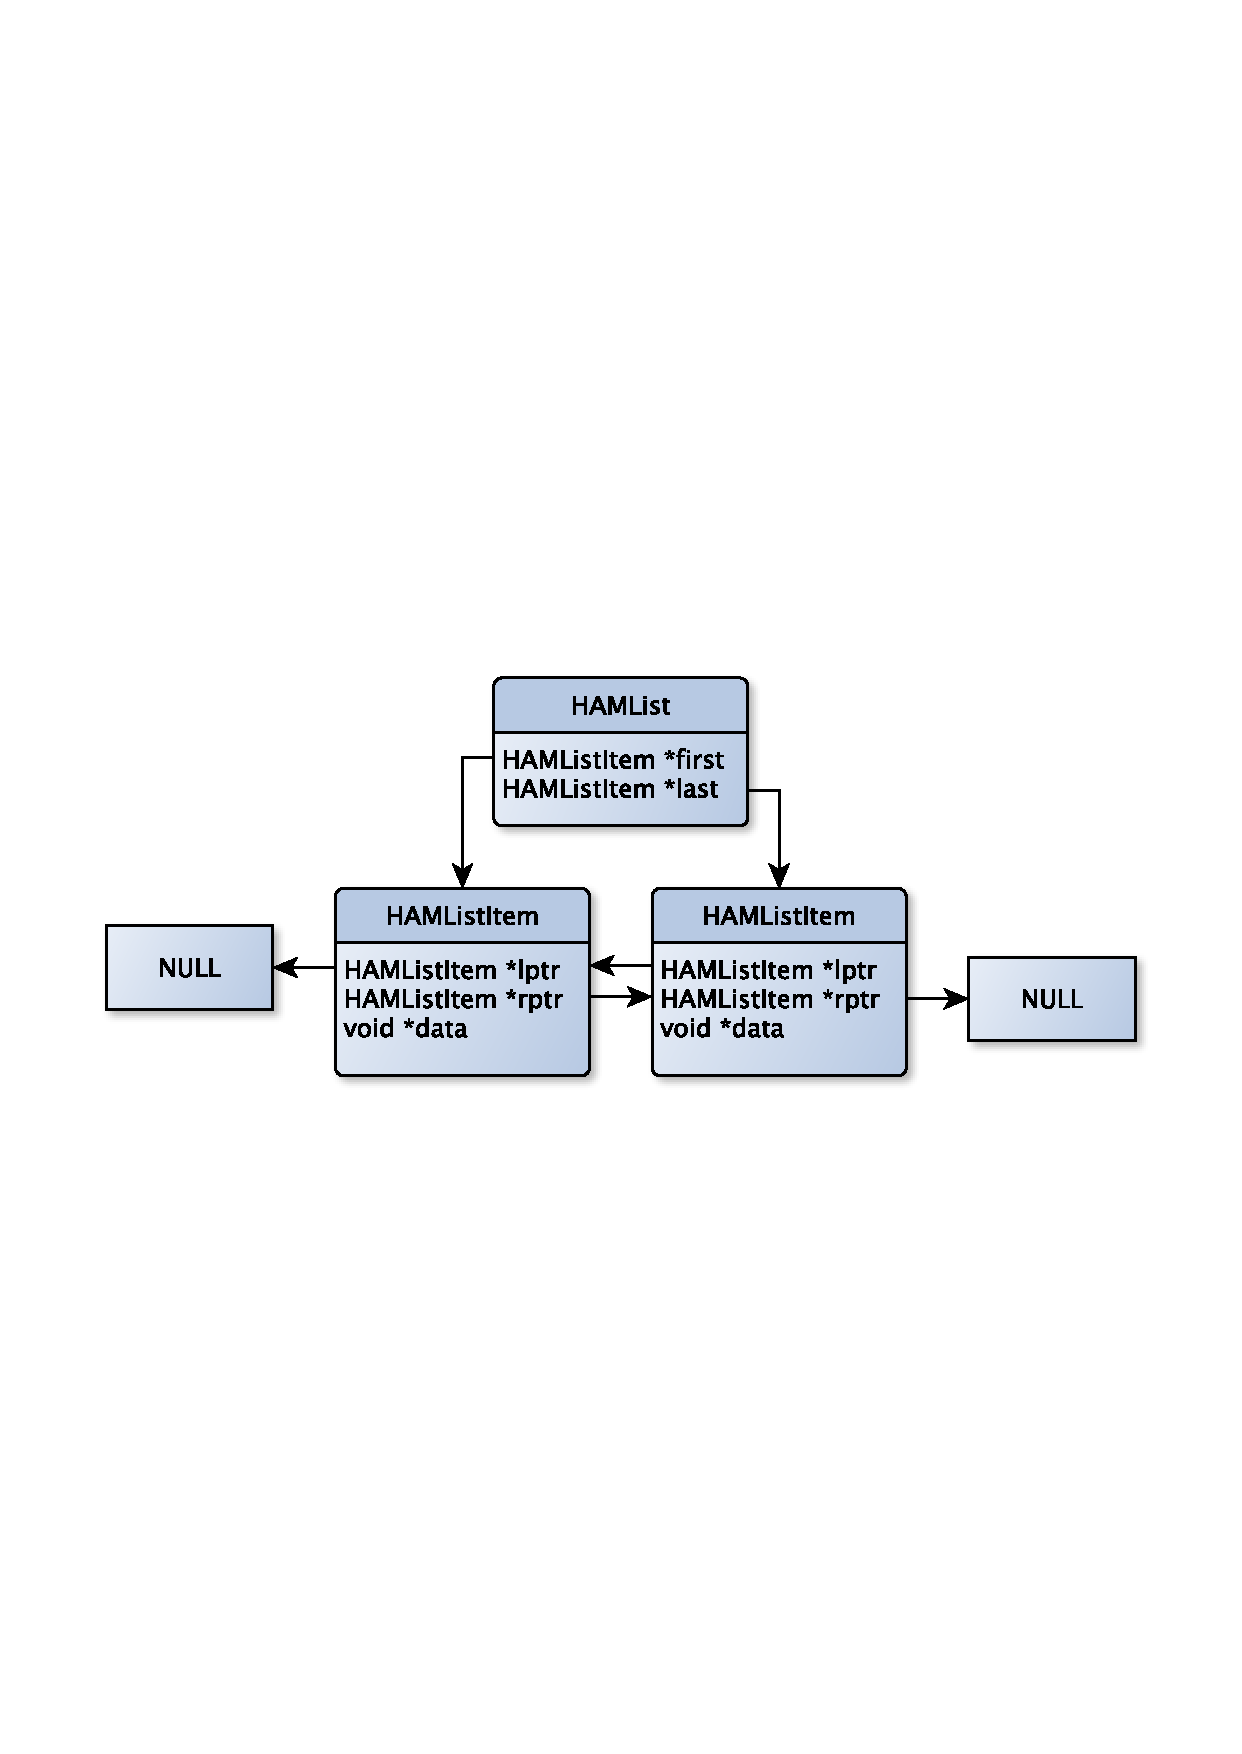
\includegraphics[trim=8cm 8cm 8cm 8cm, scale=0.6]{fig/list.pdf}
\caption{Diagram dvousm�rn�ho seznamu.}
\label{fig:FigureExample}
\end{figure}

HAMList je implementac� dvousm�rn�ho seznamu. Z�kladn� datov� struktury pou�it� pro definici seznamu jsou
HAMList a HAMListItem:

\begin{verbatim}
typedef struct _HAMListItem {
	void *data;
	struct _HAMListItem *lptr;
	struct _HAMListItem *rptr;
} HAMListItem;

typedef struct _HAMList {
	HAMListItem *first;
	HAMListItem *last;
	HAMListItemDataFree free_func;
} HAMList;
\end{verbatim}

Ka�d� polo�ka HAMListItem obsahuje odkaz na sv�ho p�edch�dce (lptr) a n�sledn�ka (rptr) a samotn� data spjat�
s polo�kou (data). Struktura HAMList obsahuje odkaz na prvn� a posledn� polo�ku a ukazatel na funkci free\_func,
kter� je pou�ita pro uvoln�n� u�ivatelsk�ch dat z pam�ti. Pokud nen� tato funkce definov�na, nejsou u�ivatelsk�
data p�i uvol�ov�n� seznamu z pam�ti uvoln�na.

\subsubsection{HAMHashTable - Hashovac� tabulka}

\begin{figure}[h]
\centering
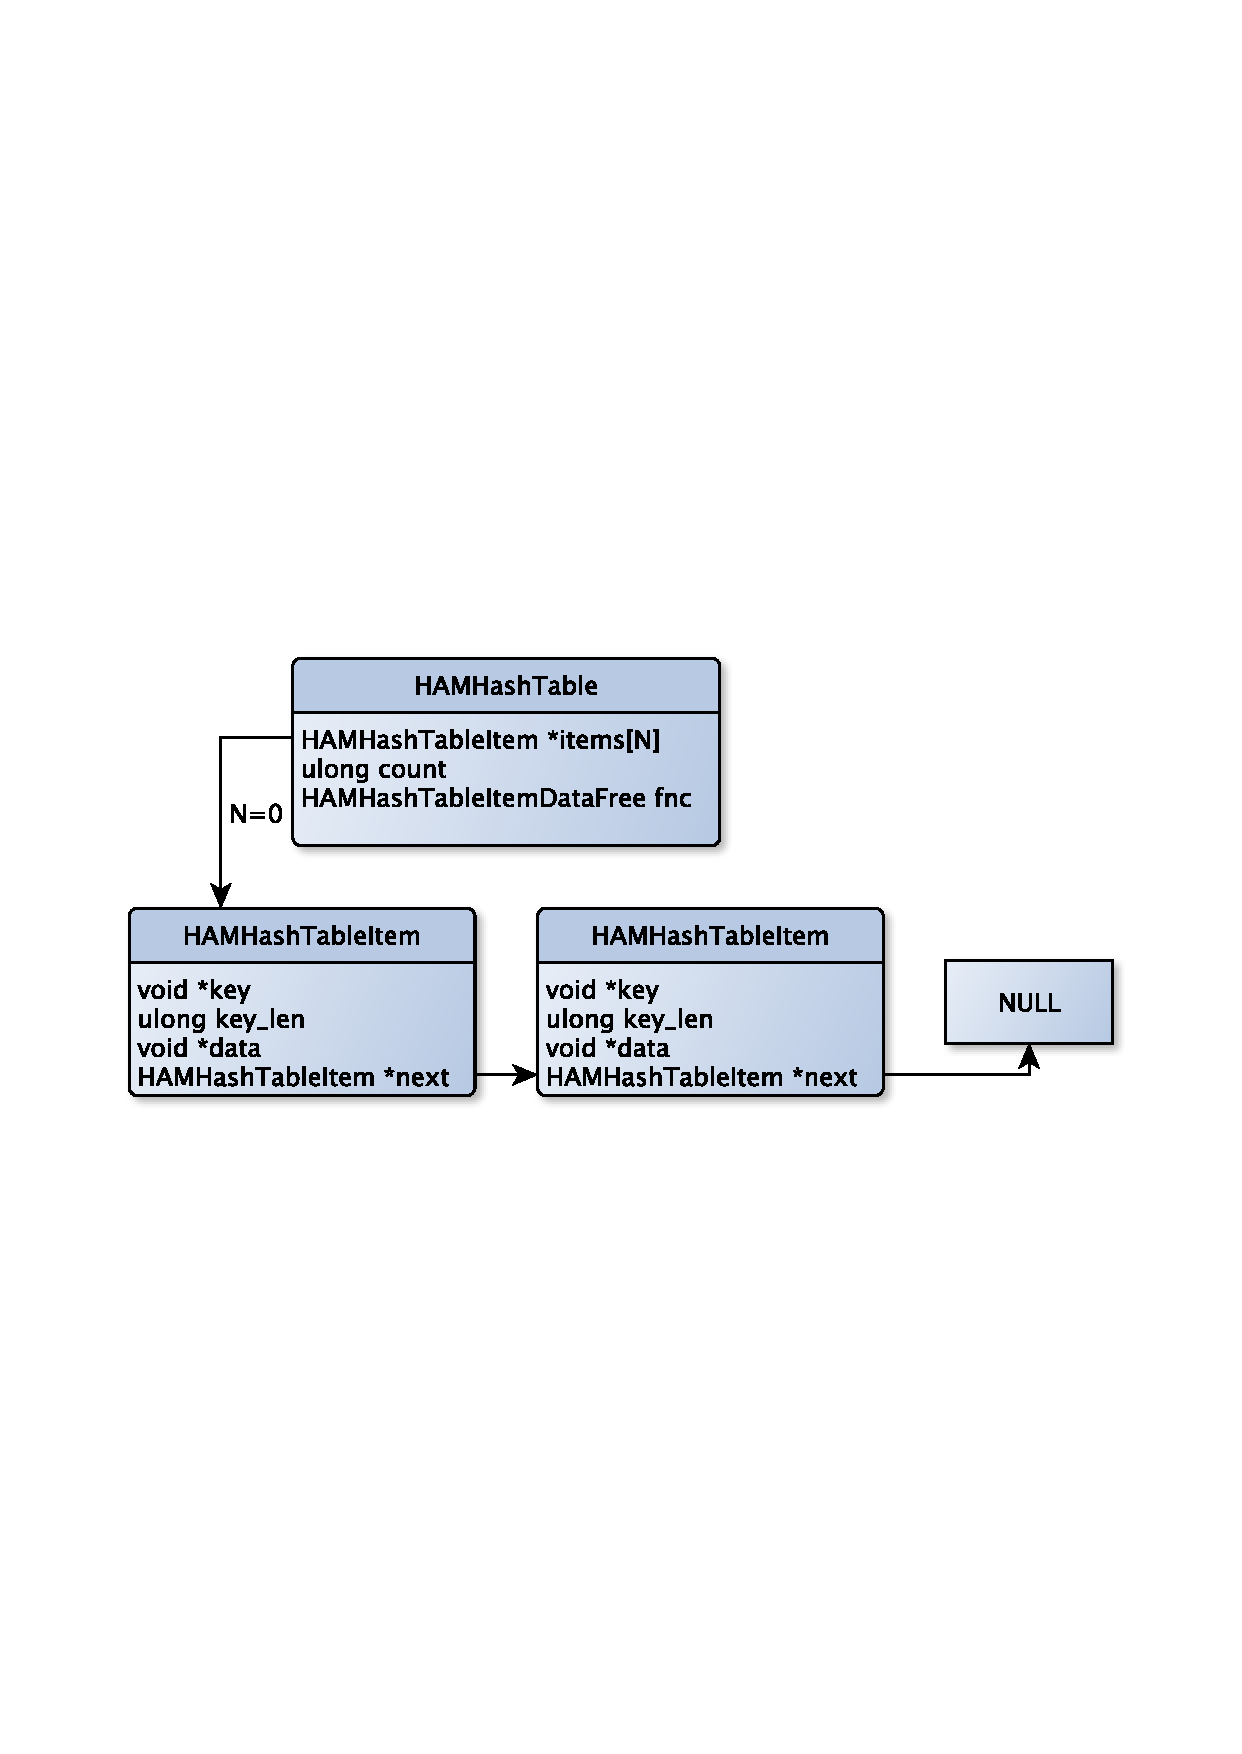
\includegraphics[trim=8cm 8cm 8cm 8cm, scale=0.6]{fig/hash.pdf}
\caption{Diagram hash tabulky seznamu.}
\label{fig:FigureExample}
\end{figure}

HAMHashTable je implementac� hash tabulky. Z�kladn� datov� struktury pou��t� p�i implementaci hash tabulky jsou
HAMHashTableItem a HAMHashTable:

\begin{verbatim}
typedef struct _HAMHashTableItem {
	const void *key;
	void *data;
	unsigned long key_len;
	struct _HAMHashTableItem *next;
} HAMHashTableItem;

typedef struct _HAMHashTable {
	HAMHashTableItem *items[HAM_HASH_LEN];
	unsigned long count;
	HAMHashTableItemDataFree free_func;
} HAMHashTable;
\end{verbatim}

Ka�d� polo�ka ulo�en� v hash tabulce obsahuje sv�j kl�� (key), jeho d�lku (key\_len), data sv�zan� s polo�kou a ukazatel
na dal�� polo�ku. P�i vlo�en� nov� polo�ky do tabulky je vypo�ten hash jej�ho kli�e pomoc� SDBM hashovac�ho algoritmu.
Na z�klad� hodnoty hashe je ukazatel na polo�ku ulo�en do pole polo�ek items. P

\subsection{Komunikace s klientskou aplikac�}

Pro komunikaci s klientskou aplikac� je podstatn� napojen� na jej� smy�ku ud�lost� a mo�nost p�ed�vat asynchronn�
v�sledky po�adavk� odeslan�ch serveru. V t�to podkapitole jsou pops�ny �e�en� obou t�chto probl�m�

\subsubsection{EventLoop}

Eventloop (neboli smy�ka ud�lost�) sdru�uje metody slou��c� k napojen� na hlavn� smy�ku
klientsk� aplikace. Pro spr�vnou funkci klientsk�
knihovny mus� klientsk� aplikace implementovat v�echny funkce definovan� ve struktu�e HAMEventLoopUICallbacks a
p�edat je klientsk� knihovn� prost�ednictv�m metody ham\_eventloop\_set\_ui\_callbacks().

Funkce definovan� ve struktu�e HAMEventLoopUICallbacks jsou pak pou��v�ny dal��mi ��stmi klientsk� knihovny na
n�sleduj�c� �innosti:

\begin{itemize}
\item timeout\_add - P�id� do hlavn� smy�ky programu b��c� v klientsk� aplikaci nov� �asoca�. Klientsk� aplikace
mus� vr�tit ukazatel na strukturu jednozna�n� identifikuj�c� �asova� a
volat opakovan� funkci p�ed�nou jakou ukazatel ve zvolen�m intervalu.
\item timeout\_remove - Odebere z hlavn� smy�ky �asova� na z�klad� jeho ukazatele na strukturu, kter� jej identifikuje.
\item input\_add - P�id� do hlavn� smy�ky klientsk� aplikace ukazatel na funkci, kter� je vol�na kdy� jsou k dispozici
nov� data na definovan�m soketu. Klientsk� aplikace
mus� vr�tit ukazatel na strukturu jednozna�n� identifikuj�c� tuto ud�lost.
\item input\_remove - Odebere z hlavn� smy�ky ukazatel na funkci vstupu na
z�klad� ukazatele na strukturu, kter� jej identifikuje.
\end{itemize}

D�ky t�to abstrakci je tak mo�no napojit klientskou knihovnu na jakoukoliv smy�ku ud�lost�.

\subsubsection{Sign�ly}

Jednotliv� ��sti klientsk� knihovny umo��uj� definovat sign�ly, na kter� se pak m��e klientsk� aplikace napojit.
Seznam sign�l� je ulo�en v hash tabulce, kde kl��em je n�zev sign�lu a daty seznam funkc�, kter� jsou zavol�ny
pokud je sign�l emitov�n. K registraci nov�ch sign�l� slou�� funkce ham\_signals\_register\_signal().

Klientsk� aplikaci je umo�n�no funkc� ham\_signals\_register\_handler() zaregistrovat funkci, kter� je zavol�na
p�i emitov�n� sign�lu. Funkce mus� b�t ve form�tu HAMFetchHandler. P�i registraci sign�lu lze rovn� definovat
ukazatel na data, kter� jsou p�i emitov�n� sign�lu zpracov�vaj�c� funkci p�ed�na. Toho lze vyu��t pro udr�ov�n�
kontextu p�i zpracov�v�n� sign�lu.


\subsection{Komunikace se serverem}

Tato podkapitola popisuje implementaci komunikace se serverem v klientsk� knihovn�. Je zde pops�no rozhran� pro
p�ipojen� k serveru, parser komunika�n�ho protokolu a pomocn� struktury Reply a Request pro reprezetanci odchoz�ch a
p��choz�ch paket�.

\subsubsection{P�ipojen� k serveru}

Pro p�ipojen� k serveru je nutn� vytvo�it novou instanci struktury Connection funkc� ham\_connection\_new(). Touto funkc�
se definuje adresa a port serveru, u�ivatelsk� jm�no a heslo. Samotn� p�ipojen� prob�hne a� po zavol�n� funkce
ham\_connection\_connect(). Tato funkce vytvo�� nov� soket pro p�ipojen� k serveru a pomoc� funkce ham\_eventloop\_input\_add()
p�id� do hlavn� smy�ky programu ukazatel na funkci pro parsov�n� p�ijat�ch dat.

\subsubsection{Parsov�n� dat}

K parsov�n� dat v klientsk� knihovn� slou�� HAMParser. TODO


\section{Implementace klientsk� aplikace}

Referen�n� klientsk� aplikace byla naprogramov�na v jazyce C++ s vyu�it�m grafick�ho frameworku Qt. V t�to kapitole jsou stru�n�
pops�ny jednotliv� t��dy klientsk� aplikace a jejich napojen� na klientskou knihovnu.




\chapter{Z�v�r}
Z�v�re�n� kapitola obsahuje zhodnocen� dosa�en�ch v�sledk� se zvlṻ vyzna�en�m vlastn�m p��nosem studenta. Povinn� se zde objev� i zhodnocen� z pohledu dal��ho v�voje projektu, student uvede n�m�ty vych�zej�c� ze zku�enost� s �e�en�m projektem a uvede rovn� n�vaznosti na pr�v� dokon�en� projekty.
 % viz. obsah.tex

  % Pouzita literatura
  % ----------------------------------------------
\ifczech
  \bibliographystyle{czechiso}
\else 
  \bibliographystyle{plain}
%  \bibliographystyle{alpha}
\fi
  \begin{flushleft}
  \bibliography{projekt} % viz. literatura.bib
  \end{flushleft}
  \appendix
  
  \chapter{Obsah CD}

\begin{itemize}
\item \textbf{./doc/} -- Programová dokumentace ke klientské knihovně (Doxygen).
\item \textbf{./latex/} -- Zdrovojé kódy technické zprávy.
\item \textbf{./src/server/} -- Zdrovojé kódy serverové aplikace.
\item \textbf{./src/library/} -- Zdrovojé kódy klientské knihovny.
\item \textbf{./src/ui/qt/} -- Zdrovojé kódy klientské aplikace.
\item \textbf{./zprava.pdf} -- Tato technická zpráva.
\item \textbf{./readme.txt} -- Návod na zprovoznění a otestování aplikace.
\end{itemize}

%\chapter{Manual}
%\chapter{Konfigrační soubor}
%\chapter{RelaxNG Schéma konfiguračního soboru}
%\chapter{Plakat}

 % viz. prilohy.tex
\end{document}
